\documentclass [tikz] {standalone}

%common figure styles
\input{header.htex}



\begin {document}		
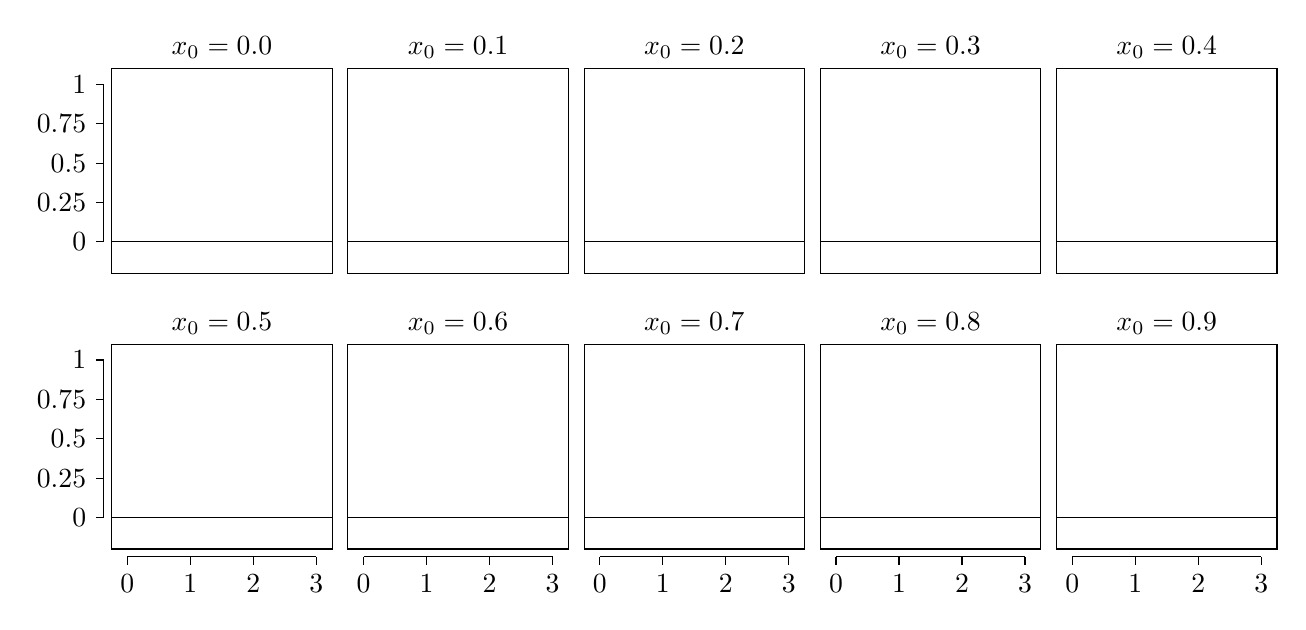
\begin{tikzpicture}		



\foreach \y in {-1,0}
{
	\foreach \x in {0,1,2,3,4}
	{
		\draw[-] (\x*3cm - 0.2cm, \y*3.5cm) -- (\x*3cm+2.6cm, \y*3.5cm);
		\draw[-] (\x*3cm - 0.2cm, \y*3.5cm - 0.4cm) rectangle (\x*3cm+2.6cm, \y*3.5cm + 2.2cm);
	}
}


\node[above] at(1.2,  2.2) {$x_0 = 0.0$};
\node[above] at(4.2,  2.2) {$x_0 = 0.1$};
\node[above] at(7.2,  2.2) {$x_0 = 0.2$};
\node[above] at(10.2, 2.2) {$x_0 = 0.3$};
\node[above] at(13.2, 2.2) {$x_0 = 0.4$};


\node[above] at(1.2,  -1.3) {$x_0 = 0.5$};
\node[above] at(4.2,  -1.3) {$x_0 = 0.6$};
\node[above] at(7.2,  -1.3) {$x_0 = 0.7$};
\node[above] at(10.2, -1.3) {$x_0 = 0.8$};
\node[above] at(13.2, -1.3) {$x_0 = 0.9$};


\foreach \x in {0,1,2,3,4}
{
	 \draw[-] (\x*3cm, -4.1cm) node[below] {$0$} -- (\x*3cm, -4cm); 
	 \draw[-] (\x*3cm + 0.8cm, -4.1cm) node[below] {$1$} -- (\x*3cm+ 0.8cm, -4cm);
	 \draw[-] (\x*3cm + 1.6cm, -4.1cm) node[below] {$2$} -- (\x*3cm+ 1.6cm, -4cm);
	 \draw[-] (\x*3cm + 2.4cm, -4.1cm) node[below] {$3$} -- (\x*3cm+ 2.4cm, -4cm);
	 
	 \draw[-] (\x*3cm, -4.0cm) -- (\x*3cm+2.4cm, -4cm);
}


\foreach \x in {0,-1}
{
	 \draw[-] (-0.4cm, \x*3.5cm) 			node[left] {$0$} 	-- (-0.3cm, \x*3.5cm) 			;
	 \draw[-] (-0.4cm, \x*3.5cm + 0.5cm) 	node[left] {$0.25$} -- (-0.3cm, \x*3.5cm + 0.5cm) 	;
	 \draw[-] (-0.4cm, \x*3.5cm + 1cm) 		node[left] {$0.5$} 	-- (-0.3cm, \x*3.5cm + 1cm) 	;
	 \draw[-] (-0.4cm, \x*3.5cm + 1.5cm) 	node[left] {$0.75$} -- (-0.3cm, \x*3.5cm + 1.5cm) 	;
	 \draw[-] (-0.4cm, \x*3.5cm + 2cm) 		node[left] {$1$} 	-- (-0.3cm, \x*3.5cm + 2cm) 	;
	 
	 \draw[-] (-0.3cm, \x*3.5cm) -- (-0.3cm, \x*3.5cm+2cm);
}




%
%\foreach \x in {-1,0}
%{
%\draw[-] (-0.75, \x*3cm) node[left]{$0$} -- (-0.5, \x*3cm) -- (-0.5, \x*3+2) -- (-0.75, \x*3+2cm) node[left]{$1$};
%\draw[-] (-0.75, \x*3+1cm) node[left]{$0.5$} -- (-0.5, \x*3+1cm);
%\draw[-] (\x*4cm+2cm, -3.75cm) node[below]{$2$} -- (\x*4cm+2cm, -3.5cm);
%}



\draw[blue] plot[ycomb, mark=*, mark options={fill=blue},mark size = 0.5mm, xshift =  0cm, yshift =  0cm] file {../dat/cm/resample_lagrange_filter_fd_time_0.0.cm};
\draw[blue] plot[ycomb, mark=*, mark options={fill=blue},mark size = 0.5mm, xshift =  3cm, yshift =  0cm] file {../dat/cm/resample_lagrange_filter_fd_time_0.1.cm};
\draw[blue] plot[ycomb, mark=*, mark options={fill=blue},mark size = 0.5mm, xshift =  6cm, yshift =  0cm] file {../dat/cm/resample_lagrange_filter_fd_time_0.2.cm};
\draw[blue] plot[ycomb, mark=*, mark options={fill=blue},mark size = 0.5mm, xshift =  9cm, yshift = 0cm] file { ../dat/cm/resample_lagrange_filter_fd_time_0.3.cm};
\draw[blue] plot[ycomb, mark=*, mark options={fill=blue},mark size = 0.5mm, xshift =  12cm, yshift = 0cm] file {../dat/cm/resample_lagrange_filter_fd_time_0.4.cm};

\draw[blue] plot[ycomb, mark=*, mark options={fill=blue},mark size = 0.5mm, xshift =  0cm, yshift =  -3.5cm] file {../dat/cm/resample_lagrange_filter_fd_time_0.5.cm};
\draw[blue] plot[ycomb, mark=*, mark options={fill=blue},mark size = 0.5mm, xshift =  3cm, yshift =  -3.5cm] file {../dat/cm/resample_lagrange_filter_fd_time_0.6.cm};
\draw[blue] plot[ycomb, mark=*, mark options={fill=blue},mark size = 0.5mm, xshift =  6cm, yshift =  -3.5cm] file {../dat/cm/resample_lagrange_filter_fd_time_0.7.cm};
\draw[blue] plot[ycomb, mark=*, mark options={fill=blue},mark size = 0.5mm, xshift =  9cm, yshift =  -3.5cm] file {../dat/cm/resample_lagrange_filter_fd_time_0.8.cm};
\draw[blue] plot[ycomb, mark=*, mark options={fill=blue},mark size = 0.5mm, xshift =  12cm, yshift = -3.5cm] file {../dat/cm/resample_lagrange_filter_fd_time_0.9.cm};



%\foreach \x in {0,1,2,3}
%{
%	\foreach \y in {0,1,2,3}
%	{
%		\draw[] (\x*5cm, -\y*3cm) rectangle (\x *5cm+4.5cm, -\y*3cm + 2cm);
%	}
%}
%	
%\foreach \x in {0,1,2,3}
%{
%	\draw[] (\x*5cm, 	-9.25cm) node[below, xshift =2mm]{$500$} -- 
%			(\x*5cm, 	-9.1cm) -- (\x*5cm+4.5cm, -9.1cm) --
%			(\x*5cm+4.5cm, -9.25cm) node[below, xshift =-2mm]{$1800$} ;
%			
%			
%	\foreach \y in {0.6819231,0.9346154,1.218462,1.526538,2.454231,2.893846,3.381923,3.921923}
%	{
%		\draw[] (\x*5cm+\y*1cm, 	-9.1cm) -- (\x*5cm+\y*1cm, -9.25cm) ;
%	}
%	
%	\draw[] (-0.1cm, 	-\x*3cm) -- (-0.1cm, -\x*3cm+2cm);
%
%	
%	\draw[] (-0.1, 	-\x*3cm) -- (-0.25, 	-\x*3cm) node[left]{$0$};
%	\draw[] (-0.1, 	-\x*3cm+2cm) -- (-0.25, 	-\x*3cm+2cm) node[left]{$120$};
%	
%	\node at (\x*5cm + 2.25cm, 	-9.7cm) [below]{$f(k)$, Гц};
%	
%	\node at (-0.7, 	-\x*3cm + 1cm) [above, rotate=90]{$|S(k)|$};	
%}	
%%{697, 770, 852, 941, 1209, 1336, 1477, 1633}
%
%\node at (2.25cm +  0cm, 2cm) [above] {\small{Символ \boxed{1}, $f = [697, 1209]$ Гц}};
%\node at (2.25cm +  5cm, 2cm) [above] {\small{Символ \boxed{2}, $f = [697, 1336]$ Гц}};
%\node at (2.25cm + 10cm, 2cm) [above] {\small{Символ \boxed{3}, $f = [697, 1477]$ Гц}};	
%\node at (2.25cm + 15cm, 2cm) [above] {\small{Символ \boxed{A}, $f = [697, 1633]$ Гц}};	
%
%\node at (2.25cm +  0cm, 2cm-3cm) [above] {\small{Символ \boxed{4}, $f = [770, 1209]$ Гц}};
%\node at (2.25cm +  5cm, 2cm-3cm) [above] {\small{Символ \boxed{5}, $f = [770, 1336]$ Гц}};
%\node at (2.25cm + 10cm, 2cm-3cm) [above] {\small{Символ \boxed{6}, $f = [770, 1477]$ Гц}};	
%\node at (2.25cm + 15cm, 2cm-3cm) [above] {\small{Символ \boxed{B}, $f = [770, 1633]$ Гц}};
%
%\node at (2.25cm +  0cm, 2cm-6cm) [above] {\small{Символ \boxed{7}, $f = [852, 1209]$ Гц}};
%\node at (2.25cm +  5cm, 2cm-6cm) [above] {\small{Символ \boxed{8}, $f = [852, 1336]$ Гц}};
%\node at (2.25cm + 10cm, 2cm-6cm) [above] {\small{Символ \boxed{9}, $f = [852, 1477]$ Гц}};	
%\node at (2.25cm + 15cm, 2cm-6cm) [above] {\small{Символ \boxed{C}, $f = [852, 1633]$ Гц}};
%
%\node at (2.25cm +  0cm, 2cm-9cm) [above] {\small{Символ \boxed{\ast}, $f = [941, 1209]$ Гц}};
%\node at (2.25cm +  5cm, 2cm-9cm) [above] {\small{Символ \boxed{0}, $f = [941, 1336]$ Гц}};
%\node at (2.25cm + 10cm, 2cm-9cm) [above] {\small{Символ \boxed{\#}, $f = [941, 1477]$ Гц}};	
%\node at (2.25cm + 15cm, 2cm-9cm) [above] {\small{Символ \boxed{D}, $f = [941, 1633]$ Гц}};
%

\end{tikzpicture}
\end {document}



